\documentclass{standalone}
\usepackage{graphicx}	
\usepackage{amssymb, amsmath, amsthm}
\usepackage{color}

\usepackage{tikz}
\usetikzlibrary{intersections, backgrounds, math}

\definecolor{light}{RGB}{220, 188, 188}
\definecolor{mid}{RGB}{185, 124, 124}
\definecolor{dark}{RGB}{143, 39, 39}
\definecolor{highlight}{RGB}{180, 31, 180}
\definecolor{darkteal}{RGB}{29, 79, 79}
\definecolor{darkolive}{RGB}{97, 123, 45}
\definecolor{gray10}{gray}{0.1}
\definecolor{gray20}{gray}{0.2}
\definecolor{gray30}{gray}{0.3}
\definecolor{gray40}{gray}{0.4}
\definecolor{gray60}{gray}{0.6}
\definecolor{gray70}{gray}{0.7}
\definecolor{gray80}{gray}{0.8}
\definecolor{gray90}{gray}{0.9}
\definecolor{gray95}{gray}{0.95}

% #1: x0
% #2: y0
% #3: R
\newcommand{\randpoints}[3]{
  ({#1 + (1 + 0.2 * rand) * #3 * (-1)},      {#2 + (1 + 0.2 * rand) * #3 * (0)})
  ({#1 + (1 + 0.2 * rand) * #3 * (-0.7071)}, {#2 + (1 + 0.2 * rand) * #3 * (+0.7071)})
  ({#1 + (1 + 0.2 * rand) * #3 * (0)},       {#2 + (1 + 0.2 * rand) * #3 * (+1)})
  ({#1 + (1 + 0.2 * rand) * #3 * (+0.7071)}, {#2 + (1 + 0.2 * rand) * #3 * (+0.7071)})
  ({#1 + (1 + 0.2 * rand) * #3 * (+1)},      {#2 + (1 + 0.2 * rand) * #3 * (0)})
  ({#1 + (1 + 0.2 * rand) * #3 * (+0.7071)}, {#2 + (1 + 0.2 * rand) * #3 * (-0.7071)})
  ({#1 + (1 + 0.2 * rand) * #3 * (0)},       {#2 + (1 + 0.2 * rand) * #3 * (-1)})
  ({#1 + (1 + 0.2 * rand) * #3 * (-0.7071)}, {#2 + (1 + 0.2 * rand) * #3 * (-0.7071)})
}

\pgfmathsetseed{12}

\begin{document}

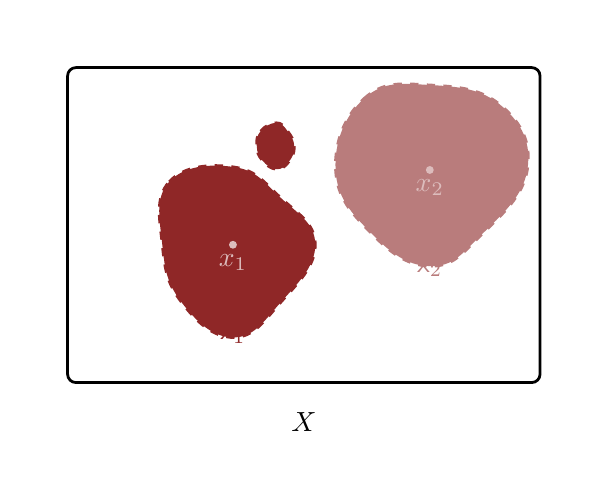
\begin{tikzpicture}[scale=1.0]
  
  \draw[white] (-3.5, -3) rectangle (3.5, 2.5);

  \draw[rounded corners=3, color=black, line width=1] (-3, -2) rectangle (3, 2);
  \node at (0, -2.5) { $X$ };

  \filldraw[dark, dashed, line width=1] 
    plot [smooth cycle, tension=0.75] coordinates { \randpoints{-0.9}{-0.25}{1} } -- cycle;
  \node[dark] at (-0.9, -1.4) {$\mathsf{x}_{1}$};
  \fill[light] (-0.9, -0.25) circle (0.05) node[below] { $x_{1}$ };
  
  \filldraw[mid, dashed, line width=1] 
    plot [smooth cycle, tension=0.75] coordinates { \randpoints{1.6}{0.7}{1.1} } -- cycle;
  \node[mid] at (1.6, -0.55) {$\mathsf{x}_{2}$};
  \fill[light] (1.6, 0.7) circle (0.05) node[below] { $x_{2}$ };
  
  \filldraw[dark, dashed, line width=1] 
    plot [smooth cycle, tension=0.75] coordinates { \randpoints{-0.35}{1}{0.25} } -- cycle;
    
\end{tikzpicture}

\end{document}  